%FOR PDFLATEX USE ONLY
\documentclass[a4paper,12pt]{article}

\usepackage{amssymb,amsmath} %math symbols

\usepackage[margin=2cm]{geometry} %paper geometry

\usepackage[utf8]{inputenc} %allows unicode (including russian) source file
\usepackage[russian]{babel} %docment in russian-style
\usepackage[utf8]{inputenc}
%\usepackage[unicode]{hyperref} %links inside of the text
\usepackage[pdftex]{graphicx} %includegraphics pictures
\usepackage{cmlgc} %bold text

\usepackage{array} %arrays

%\usepackage{wrapfig}
%\usepackage{array}
%\usepackage{lipsum}
%\usepackage{esvect}
%\usepackage{hyperref}

\usepackage{subfig}
%\usepackage{calc}
%\usepackage{pgfplots,tikz,circuitikz}
%\usepackage{tkz-euclide}
\usepackage{booktabs}
\usepackage{multirow}
\usepackage{float}

\usepackage{wrapfig}

\graphicspath{{pictures}}

\begin{document}

\begin{center}
  \LARGE{Работа 4.7.3}\\[0.2cm]
  \LARGE{Изучение поляризованного света}\\[0.2cm]
  \large{Балдин Виктор}\\[0.2cm]
\end{center}

\textbf{Цель работы}: ознакомление с методами получения и анализа поляризованного света.


\textbf{В работе используются}: оптическая скамья с осветителем; зеленый светофильтр; два поляроида; черное зеркало; полированная эбонитовая пластинка; стопа стеклянных пластинок; слюдяные пластинки разной толщины; пластинки в $1/4$ и $1/2$ длины волны; пластинка в одну длины полны для зеленого цвета (пластинка чувствительного оттенка).
\section*{Теория}

При помощи специальных приспособлений (поляризаторов), естественный свет может быть превращен в линейно поляризованный (или, как иногда говорят, в плоскополяризованный). В линейно поляризованной световой волне пара векторов \textbf{E} и \textbf{H} не изменяет с течением времени своей ориентации. Плоскость \textbf{E, S} называется в этом случае \textit{плоскостью колебаний}. \par
Наиболее общим типом поляризации является \textit{эллиптическая поляризация}. В эллиптически поляризованной световой волне конец вектора
\textbf{E} (в данной точке пространства) описывает некоторый эллипс. Линейно
поляризованный свет можно рассматривать как частный случай эллиптически поляризованного света, когда эллипс поляризации вырождается в отрезок прямой линии; другим частным случаем является круговая
поляризация (эллипс поляризации является окружностью). \par
Для получения линейно поляризованного света применяются специальные оптические приспособления — поляризаторы. Направление колебаний электрического вектора в волне, прошедшей через поляризатор, называется
разрешенным направлением поляризатора.
Всякий поляризатор может быть использован для исследования поляризованного света, т. е. в качестве анализатора. Интенсивность I линейно поляризованного света после прохождения через анализатор зависит от угла, образованного плоскостью колебаний с разрешенным направлением анализатора:
\begin{equation}
  I = I_0 \cos^2\alpha.
\end{equation}
Соотношение (1) носит название \textit{закона Малюса}. \par
. Отраженный от диэлектрика свет всегда частично поляризован. Степень поляризации света, отраженного от диэлектрической пластинки в воздух, зависит от показателя преломления диэлектрика $n$ и от угла падения $\alpha$. Как следует из формул Френеля, полная поляризация отраженного света достигается
при падении под \textit{углом Брюстера}, который определяется соотношением
\begin{equation}
 \tg \alpha = n.
\end{equation}

В этом случае плоскость колебаний электрического вектора в отраженном свете перпендикулярна плоскости падения. Для увеличения степени поляризации преломлённого
света используют стопу стеклянных пластинок, расположенных под углом Брюстера к падающему свету.

\section*{Результаты и обработка}
\subsection*{Определение разрешенных направлений поляроидов}
Разместим на оптической скамье осветитель $S$, поляроид $P$ и черное зеркало. Методом последовательных приближений найдем такое расположение поляроида и зеркала, что интенсивность отраженного света минимальна.

\begin{figure}[H]
\centering
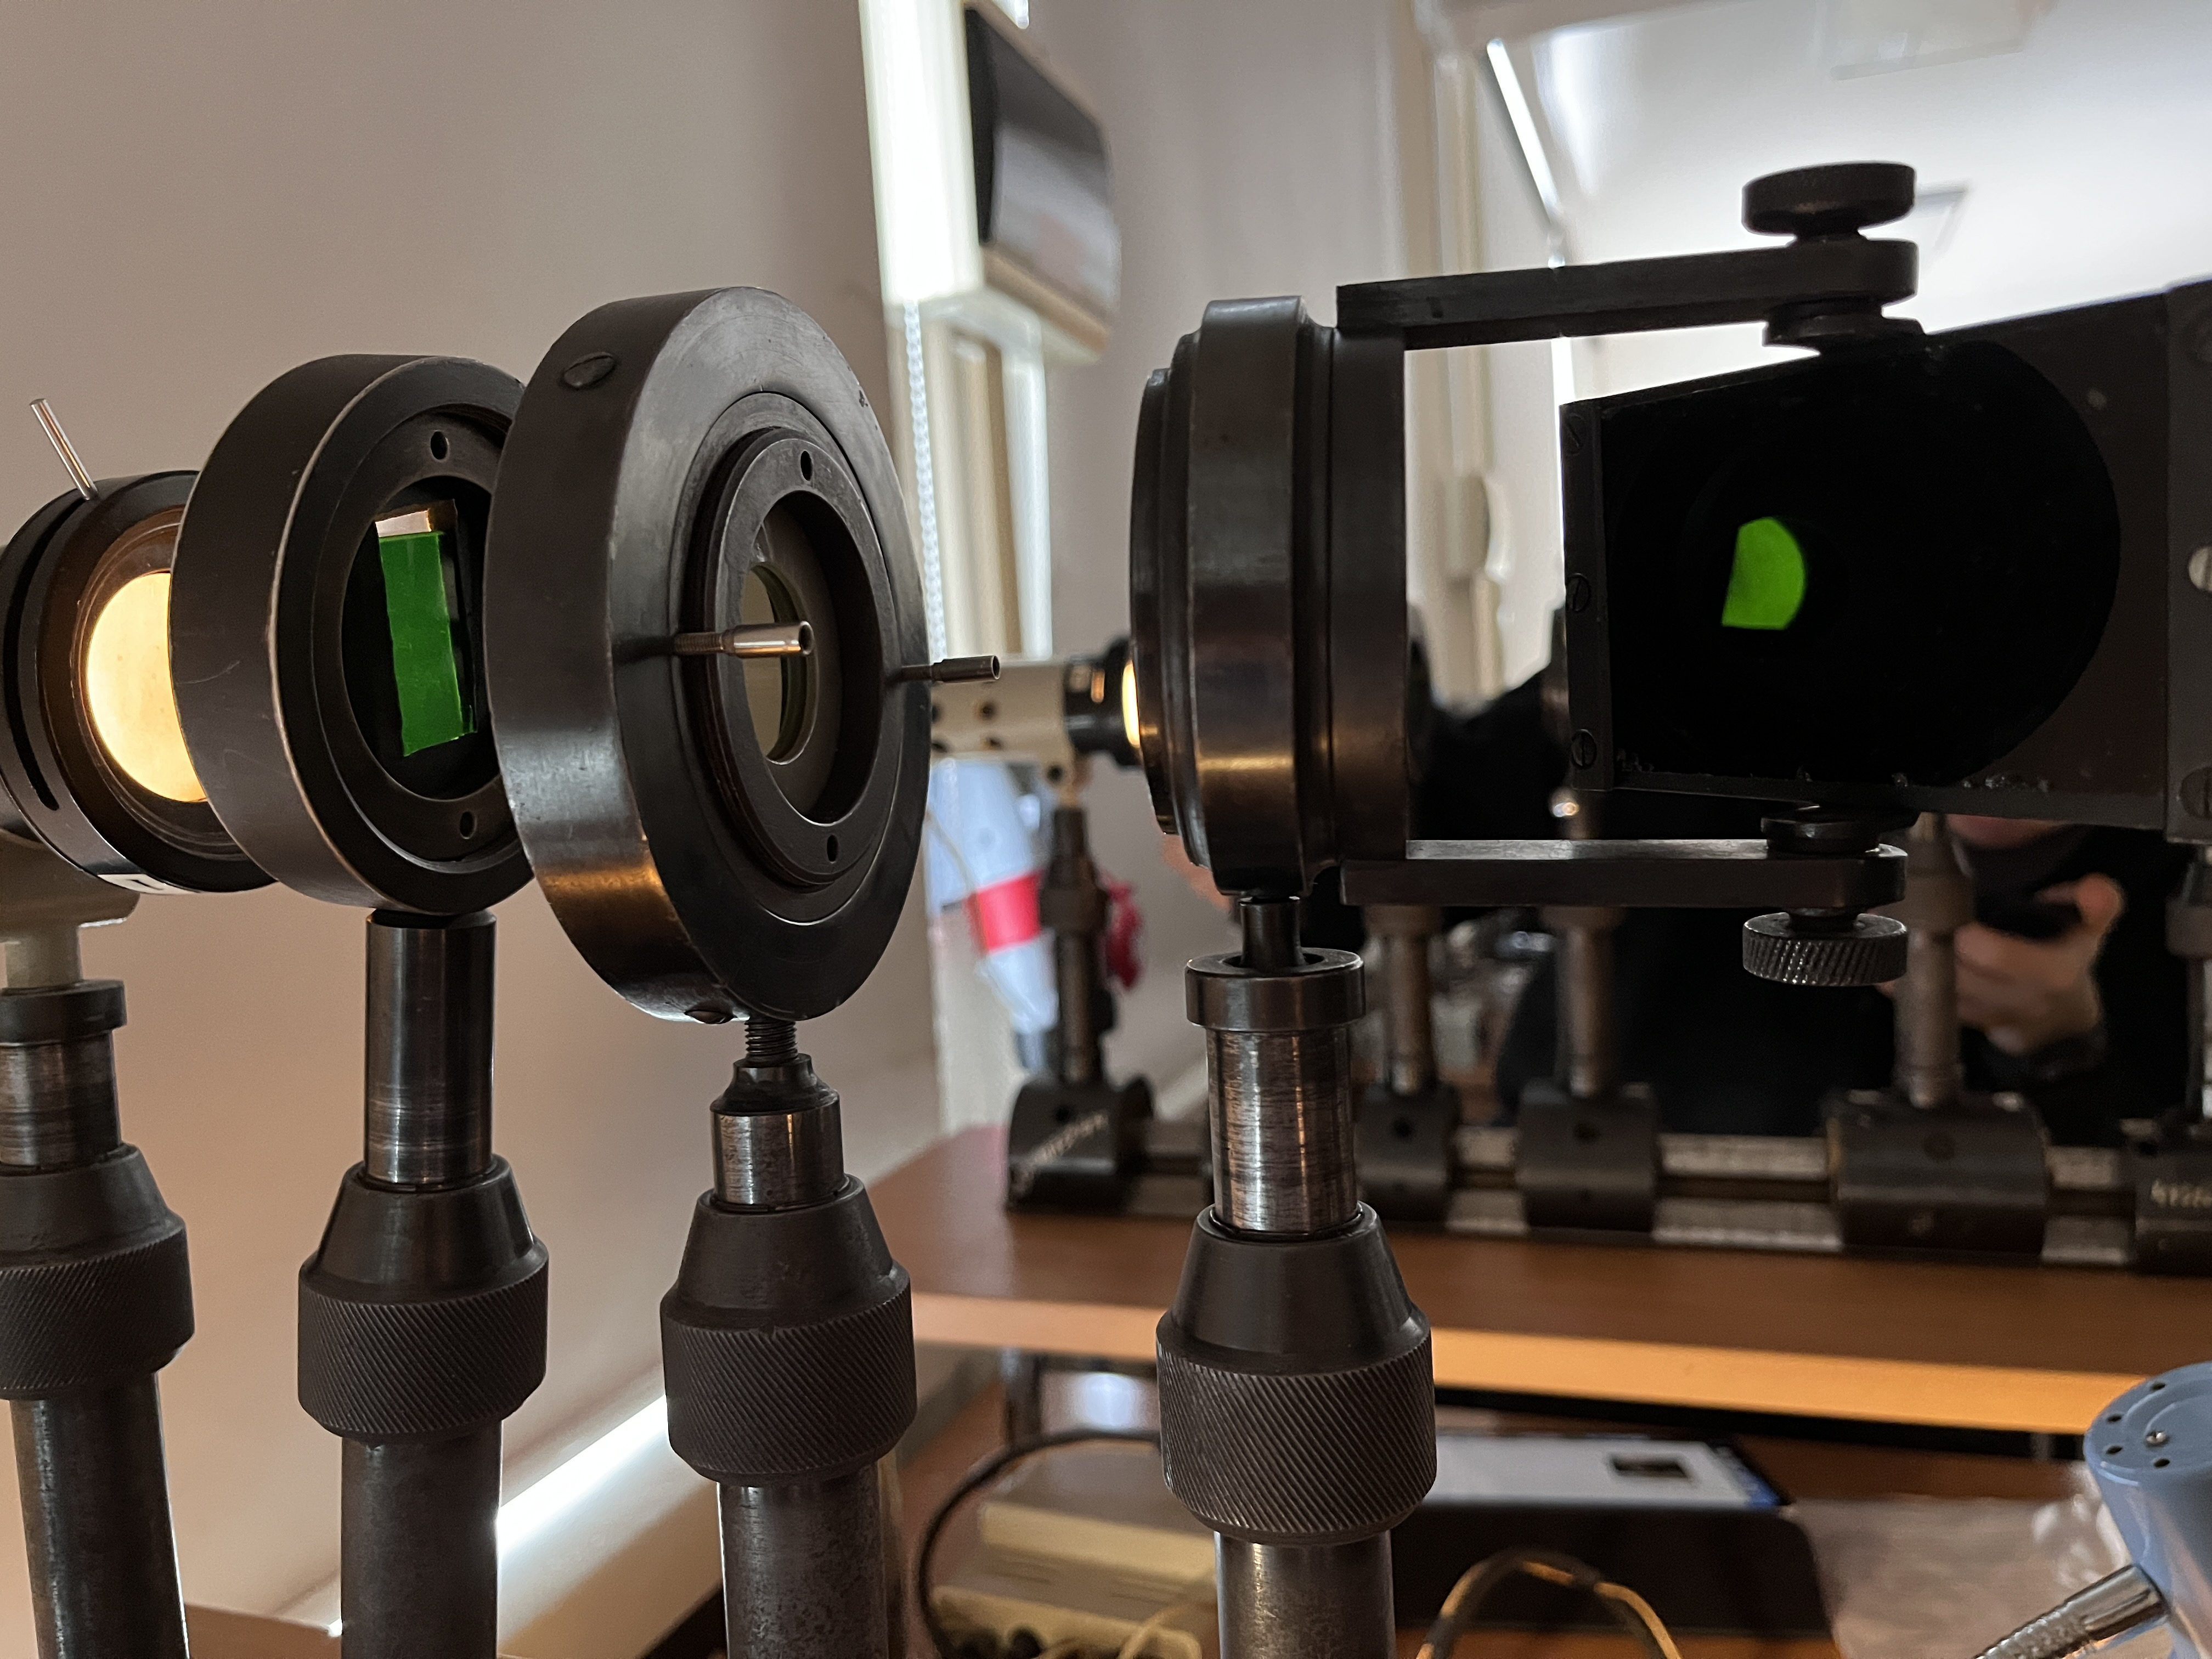
\includegraphics[width=0.80\textwidth]{IMG_3187.JPG}
\caption{Изображение источника в зеркале}
\end{figure}

Разрешенное направление второго поляроида можно определить, скрестив поляроиды.

\subsection*{Определение угла Брюстера для эбонита}
Найдем показатель преломления эбонита. Для этого посмотрим на свет источника $S$, отраженный от эбонитовой пластинки. Меняя угол поворота пластинки, добьемся того, чтобы интенсивность света после прохождения через поляризатор была минимальна. Это будет означать, что свет падает под углом Брюстера $\alpha = arctan(n)$

В результате получается значение

\[n=\tan((60 \pm 5)^\circ)=1.4\pm0.3.\]

\subsection*{Исследование стопы}
Происследуем стопу. Поставим стопу стеклянных пластинок вместо эбонитового зеркала и добьемся того, чтобы свет падал на стопу под углом Брюстера.

\begin{figure}[H]
\centering
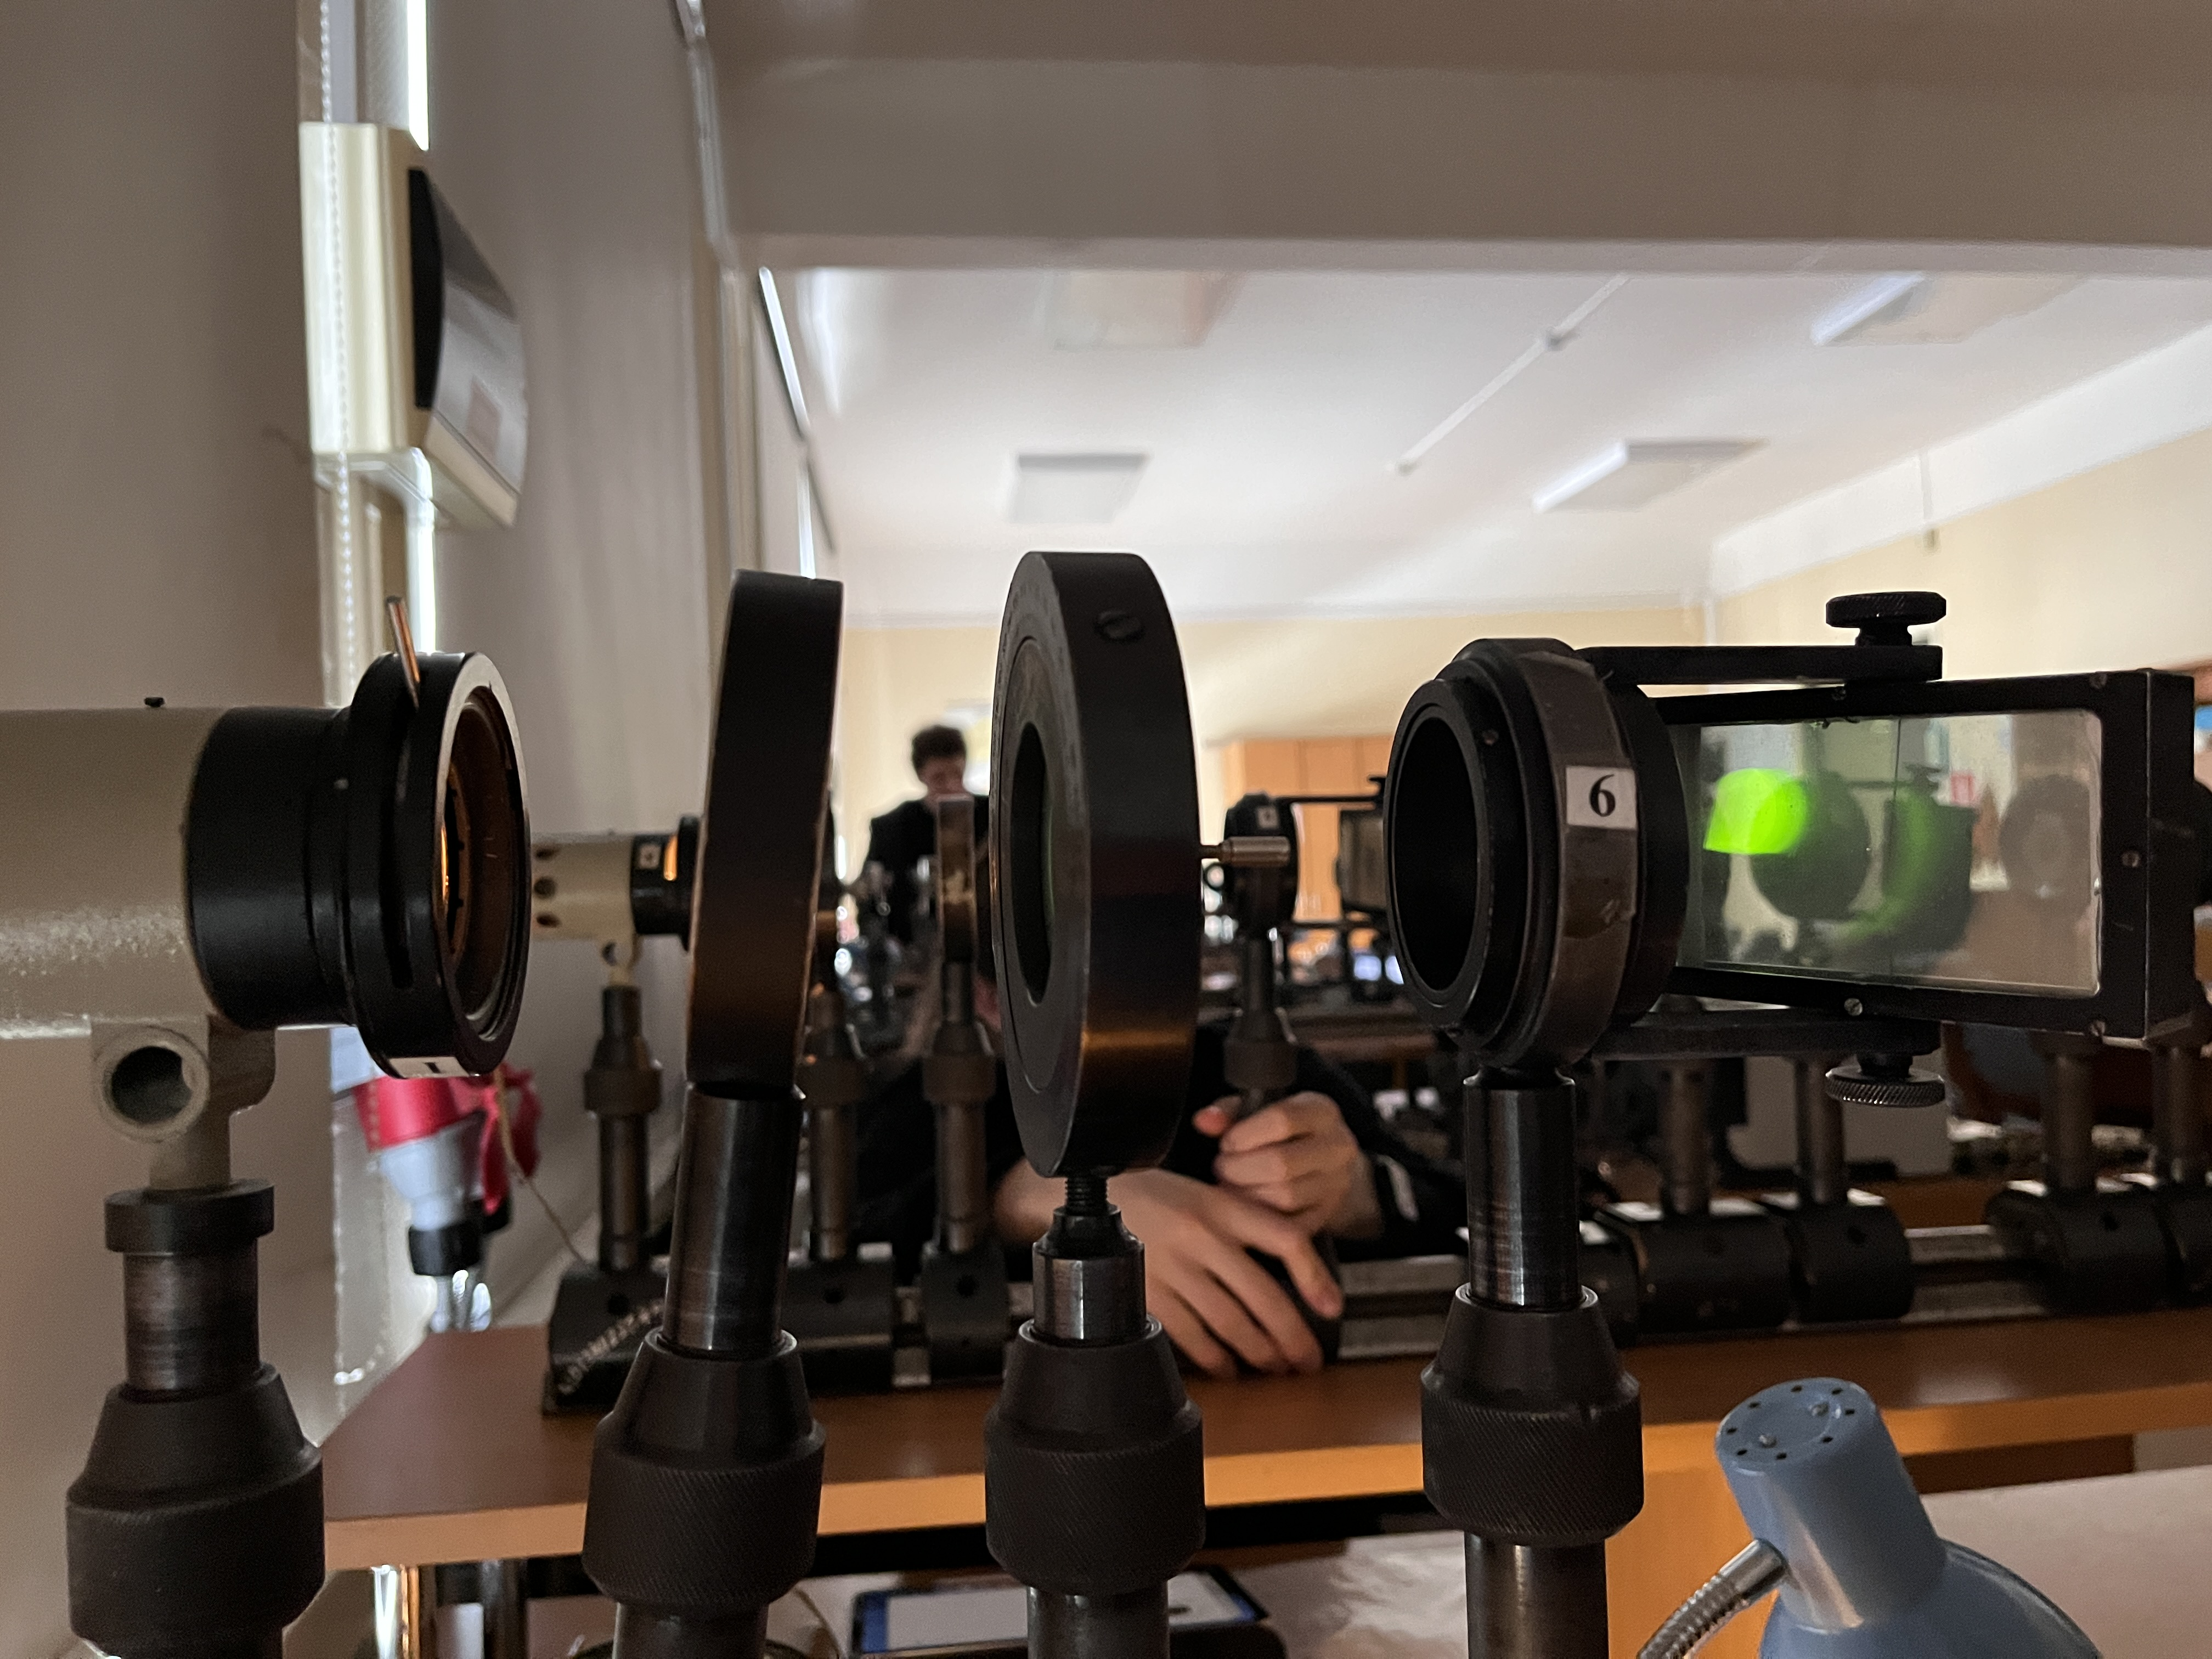
\includegraphics[width=0.80\textwidth]{IMG_3192.JPG}
\caption{Исследование стопы}
\end{figure}

Происследуем свет, отраженный и прошедший через стопу с помощью поляризаторов. Получим, что свет, отраженный от стопы поляризован вертикально, а прошедший через стопу --- горизонтально.

\subsection*{Определение главных плоскостей двоякопреломляющих пластин}

Поставим клисталлическую пластинку между скрещенными поляроидами $P_1$ и $P_2$. И происследуем интенсивность света, прошедшего через систему от угла поворота пластинки. В момент, когда главные оси совпадают с плоскостями поляроидов, интенсивность минимальная. Это происходит 4 раза за поворот.



\begin{center}
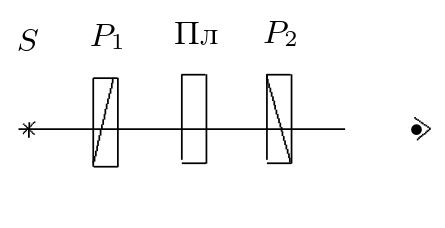
\includegraphics[width=0.50\textwidth]{5.png}\\
Определение главных направлений в пластинках
\end{center}

\subsection*{Выделение пластин $\lambda/2$ и $\lambda/4$}
Если добавить к схеме выше зеленый фильтр и повернуть главные направления в пластинке на угол $45^\circ$, то можно будет определить тип пластинки по поляризованности света, выходящего из неё. Происследуем зависимость интенсивности света, проходящего через установку, от угла поворота последнего поляризатора $P_2$. Если пластинка $\lambda/2$, свет поляризуем линейно и минимумы интенсивности наблюдаются 2 раза за оборот. Если пластинка $\lambda/4$, то минимумы интенсивности не наблюдаются из-за того, что свет имеет круговую поляризацию.

\subsection*{Выделение <<быстрой>> и <<медленной>> оси в пластинке $\lambda/4$}
Поставим между скрещенными поляроидами пластинку чувствительного оттенка, имеющую вид стрелки, и убедимся, что эта пластинка не меняет поляризацию зелёного света.

\begin{figure}[H]
  \centering
  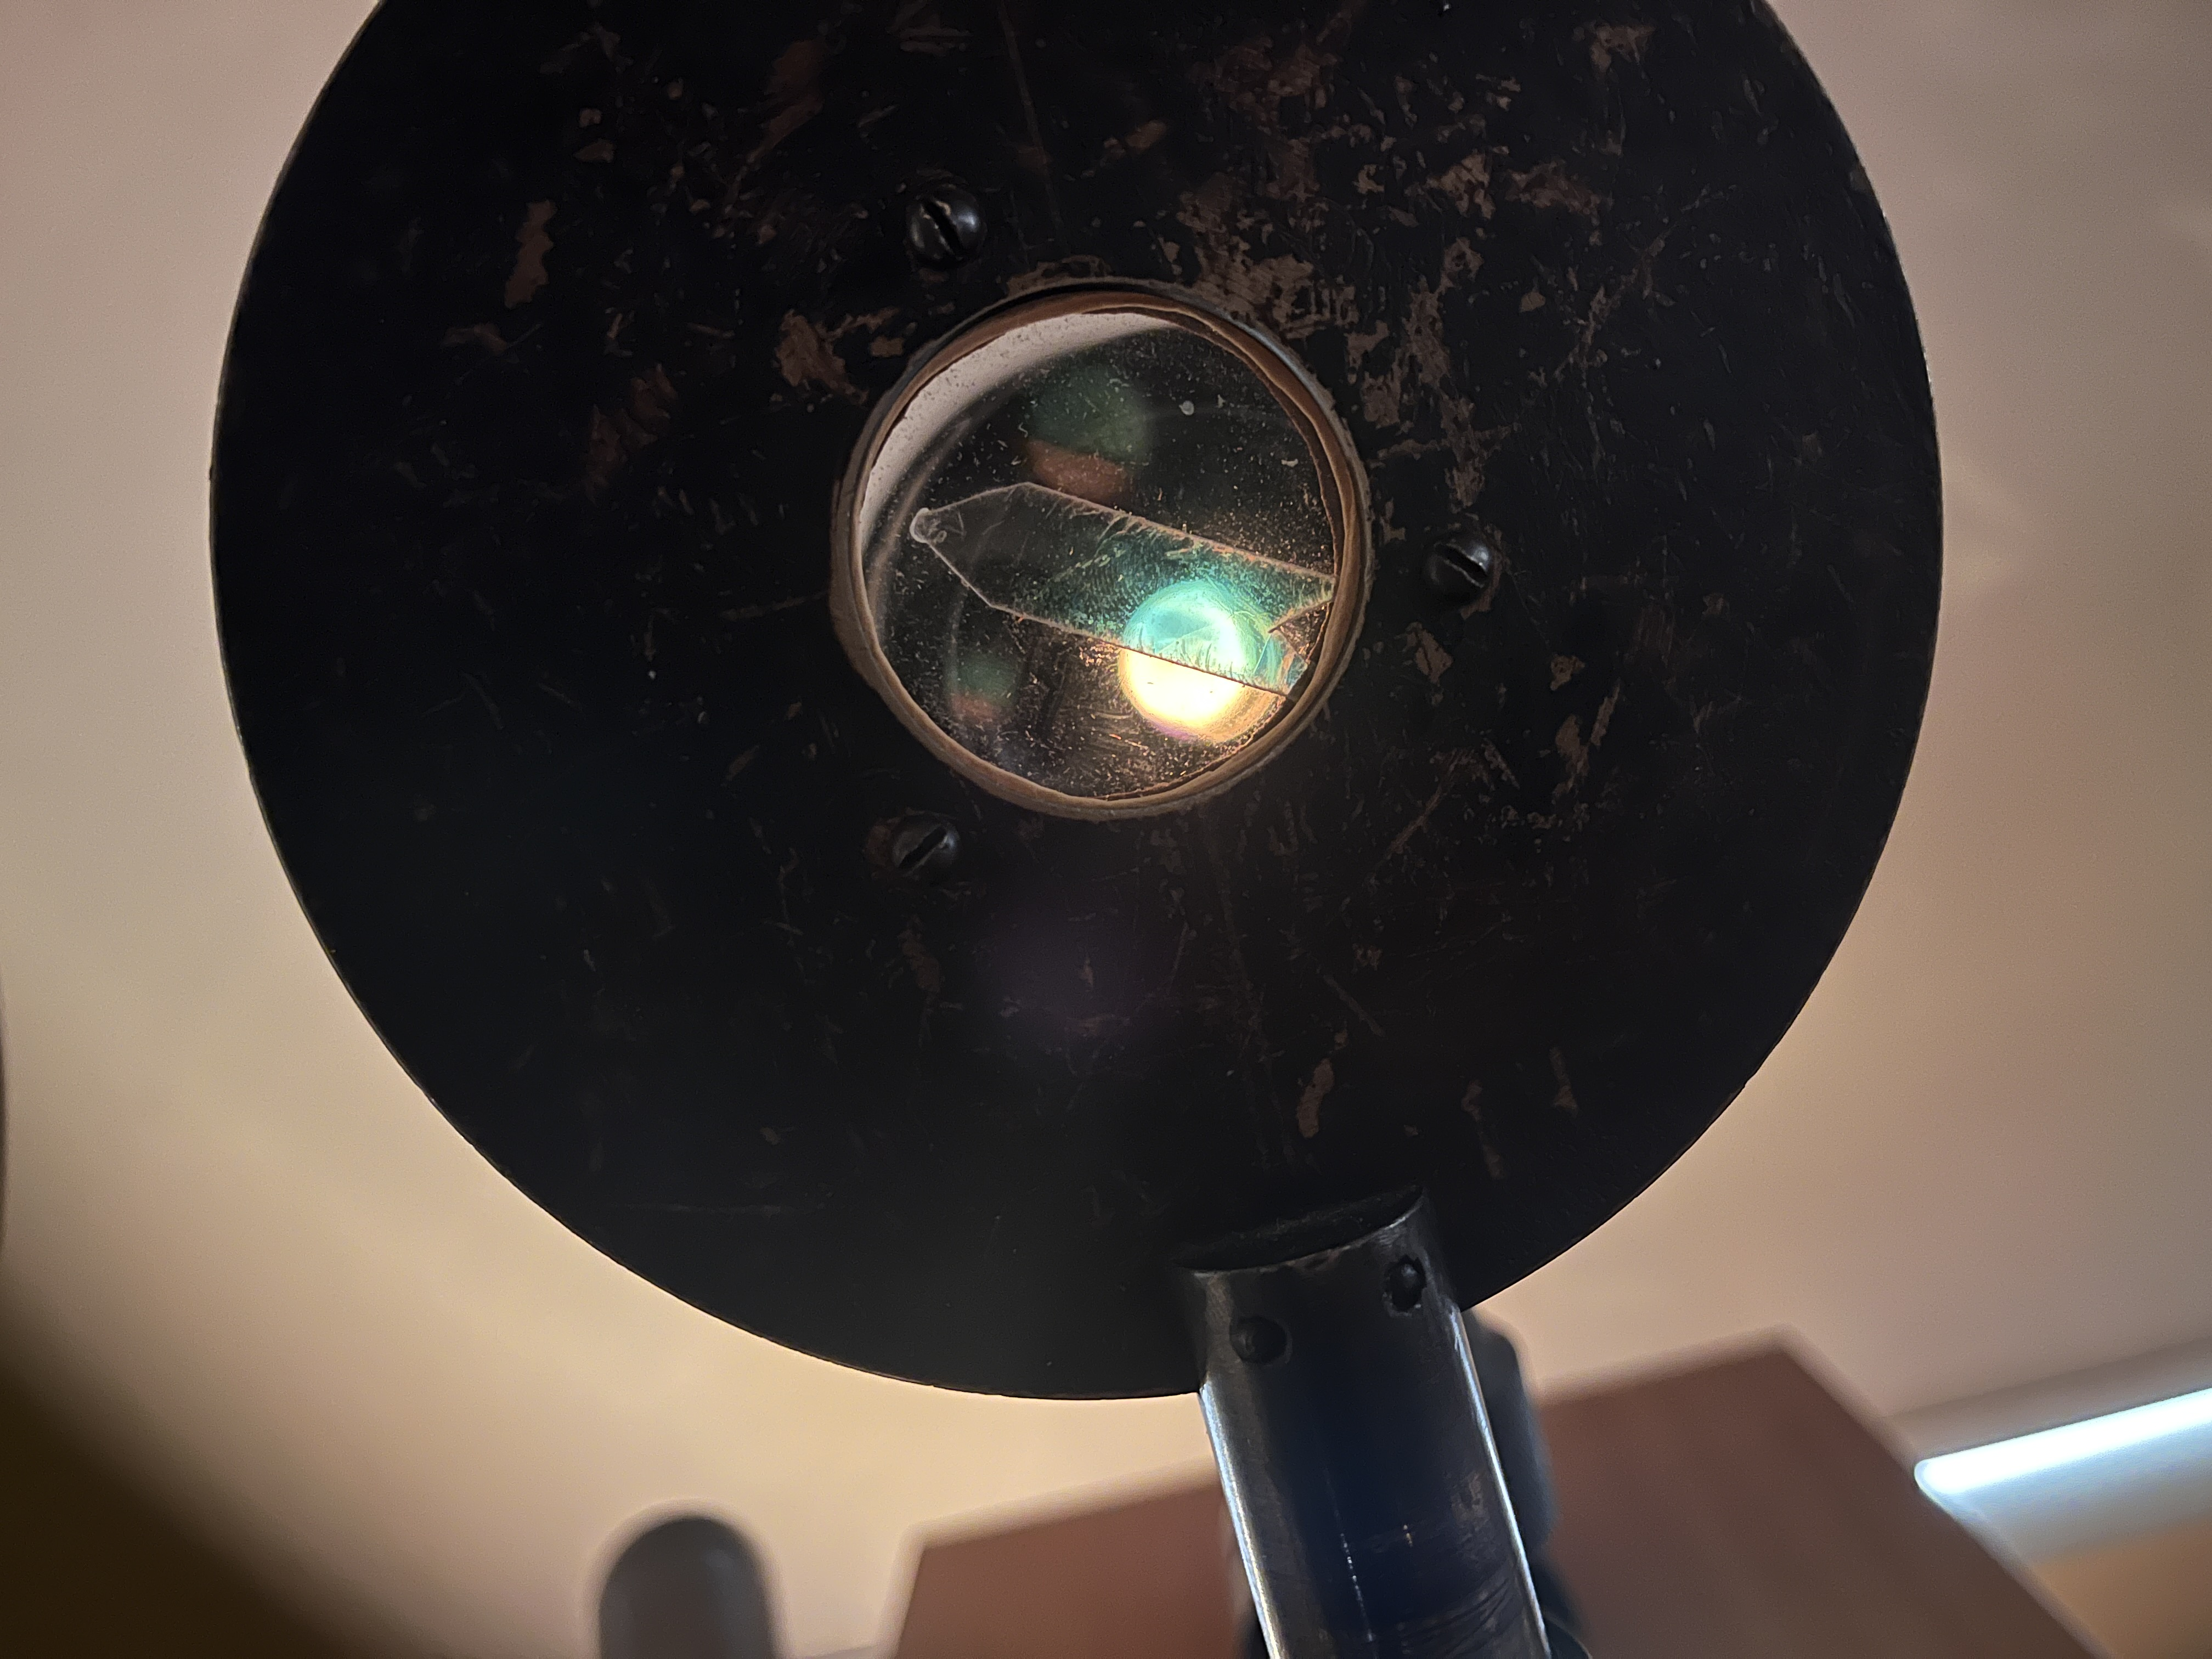
\includegraphics[width=0.8\textwidth]{IMG_3196.JPG}
  \caption{Зелено-голубой цвет пластинки}
\end{figure}

\begin{figure}[H]
  \centering
  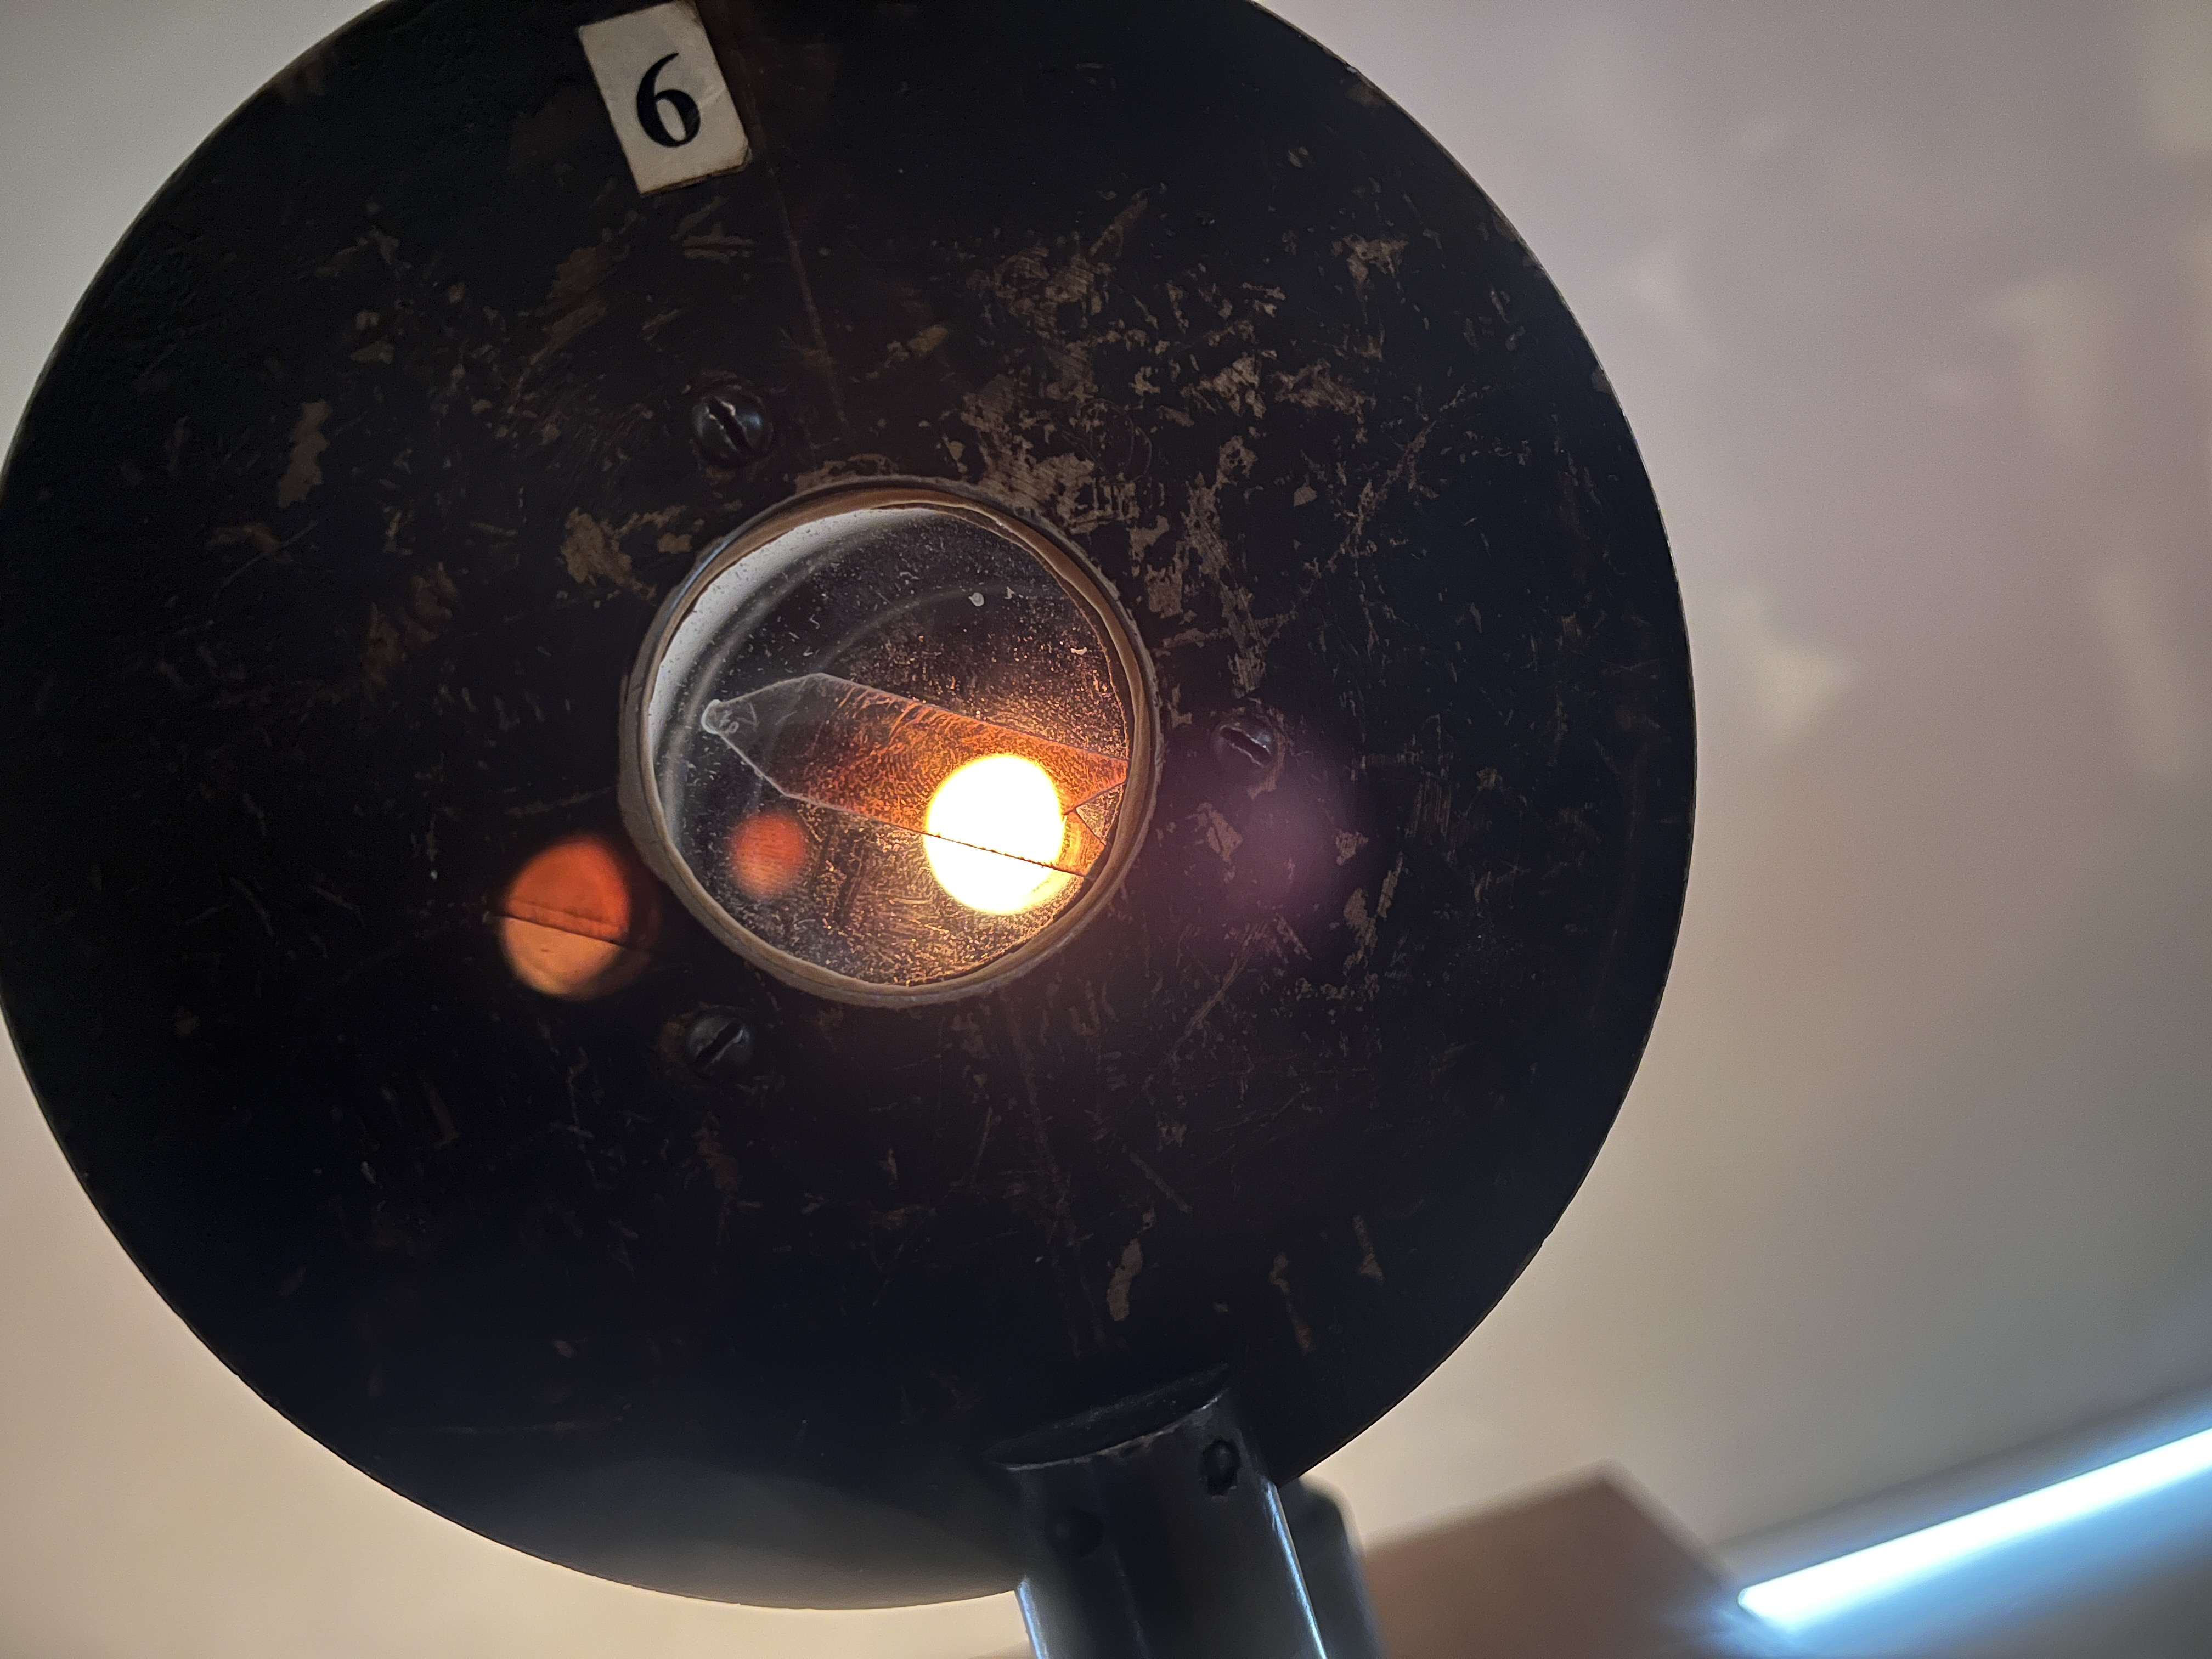
\includegraphics[width=0.8\textwidth]{IMG_3197.JPG}
  \caption{Оранжево-желтый цвет пластинки}
\end{figure}

\subsection*{Интерференция поляризованных лучей}
Расположим между скрещенными поляроидами мозаичную слюдяную пластинку. Из описания лабораторной работы следует, что пластинка состоит из 4-х узких полосок слюды, лежащих по сторонам квадрата (две полоски $\lambda/4$, одна $\lambda/2$ и еще одна $3\lambda/3$).

\begin{figure}[H]
\centering
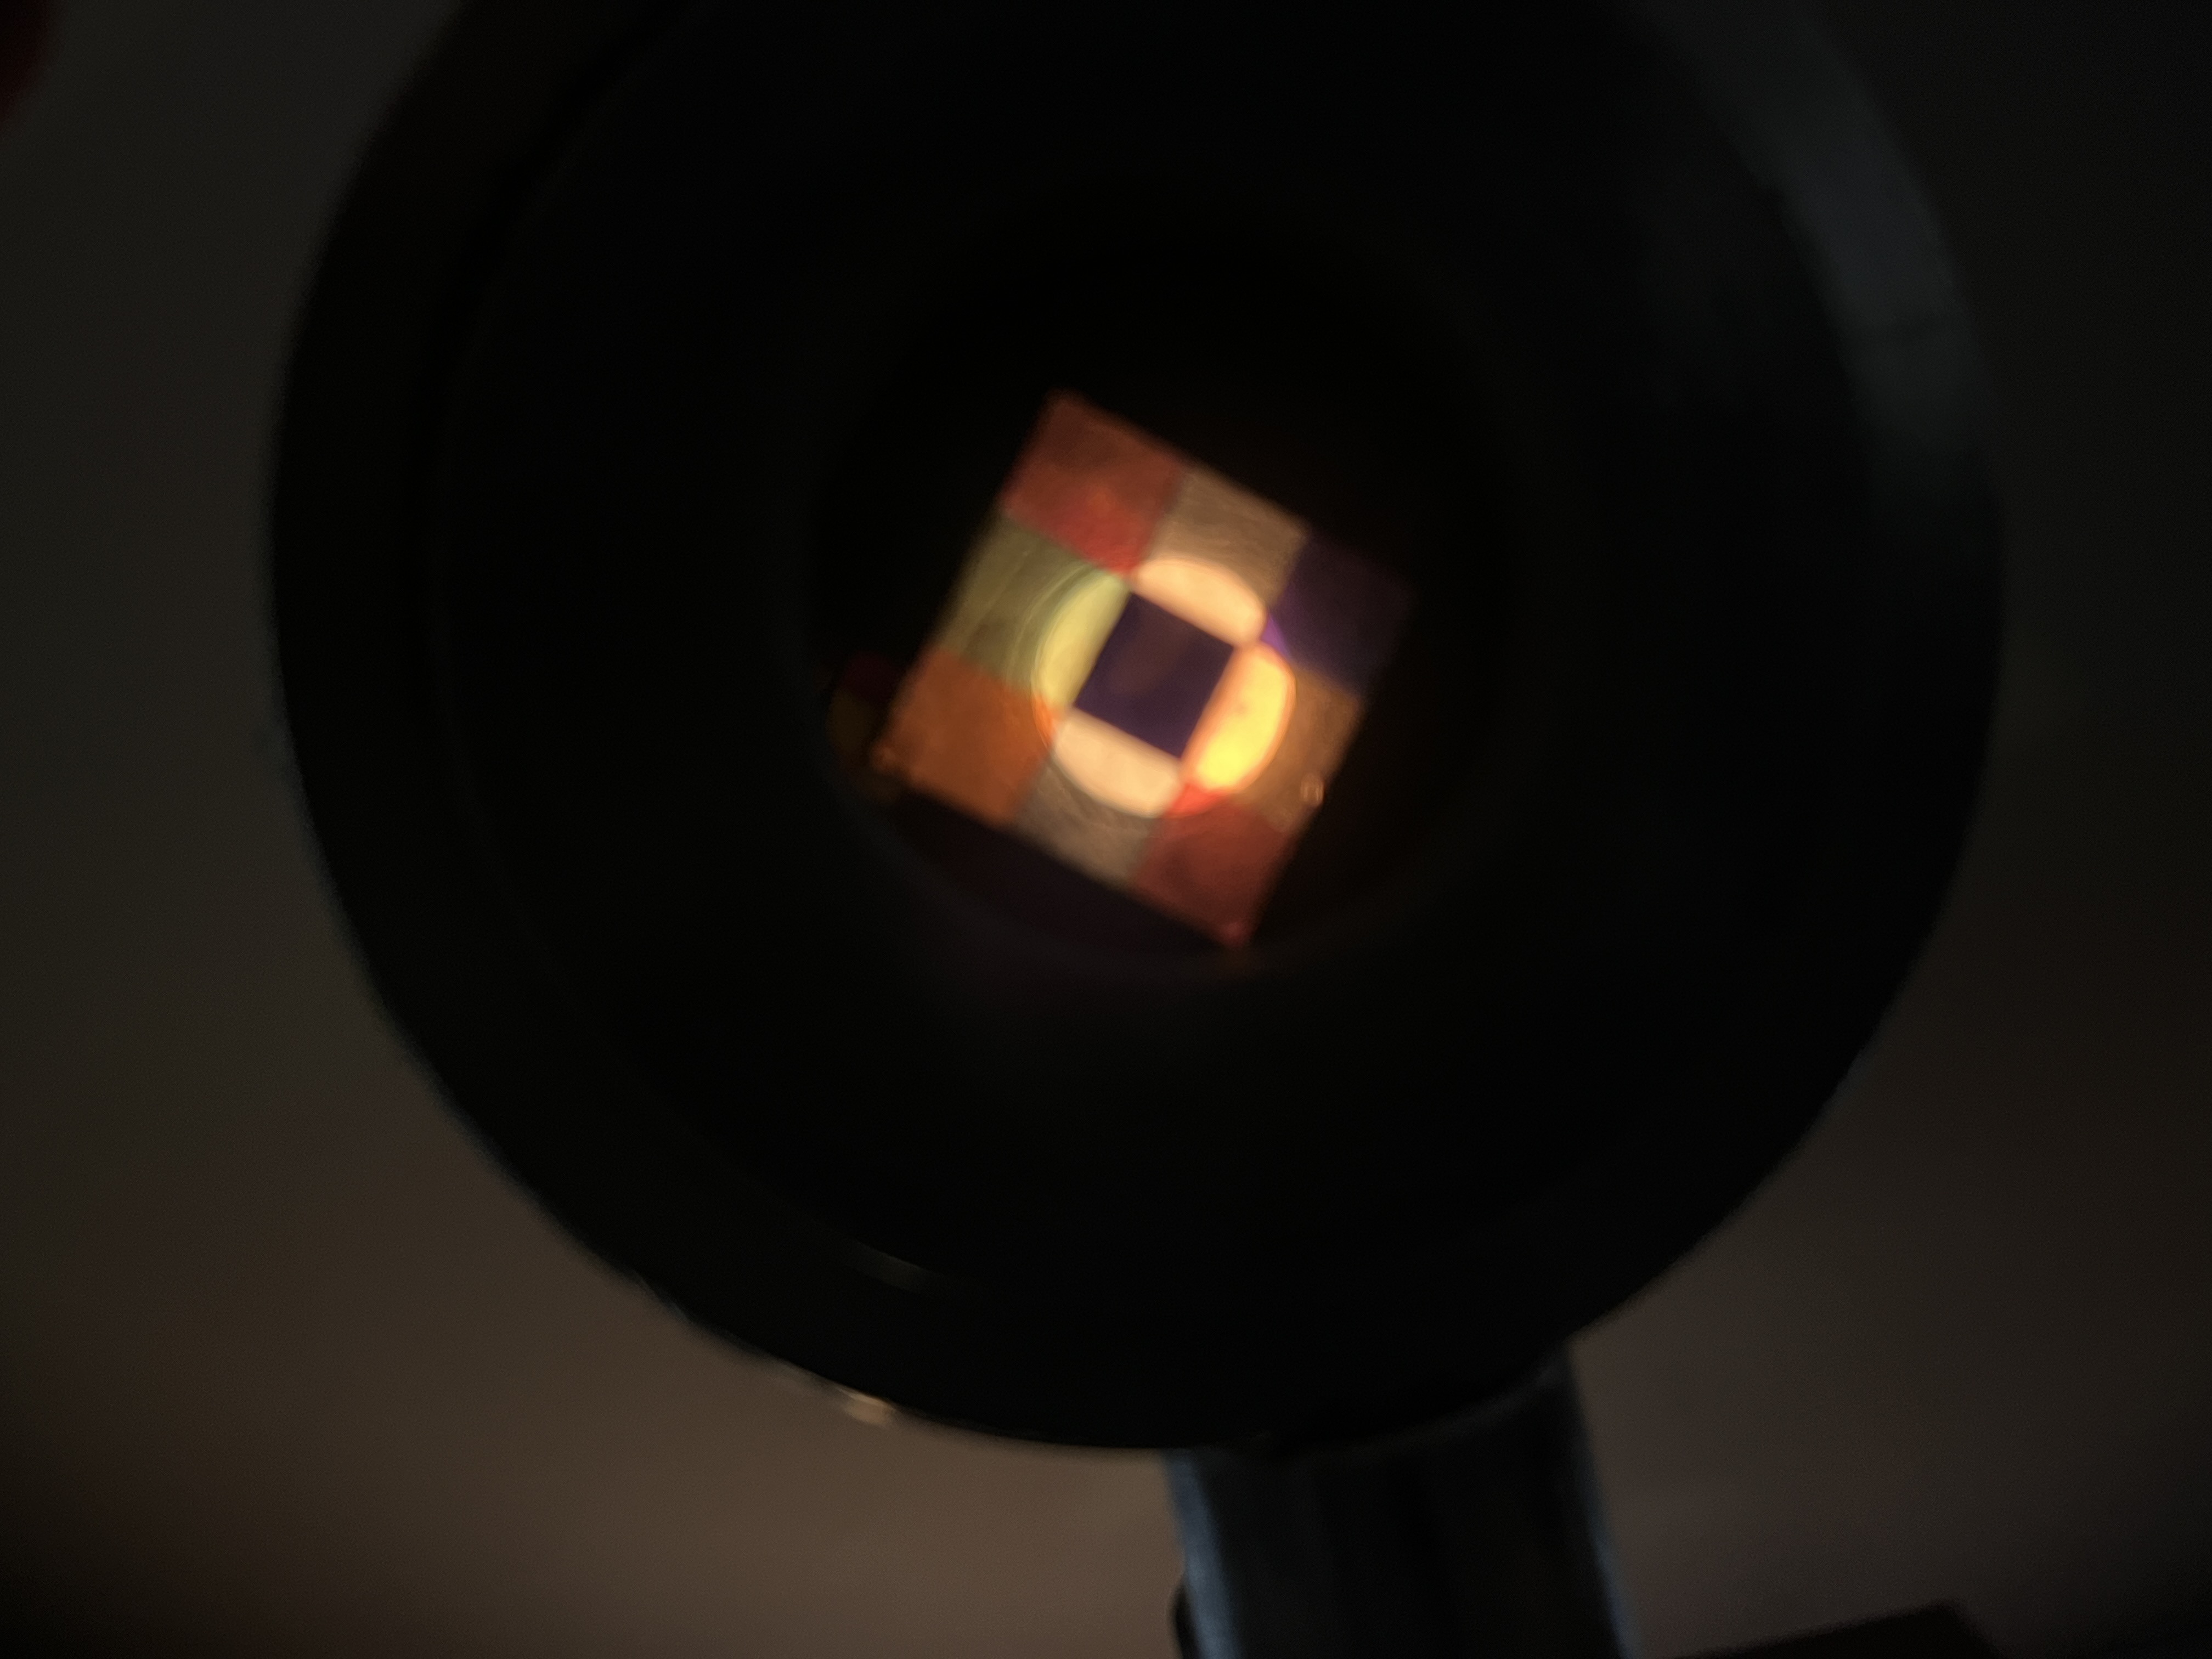
\includegraphics[width=0.80\textwidth]{IMG_3198.JPG}
\caption{Мозаичная пластинка}
\end{figure}

Эксперимент показывает, что, если вращать пластинку, интенсивность света меняется с периодом в четверть оборота. Это происходит из-за того, что 4 раза за оборот оси пластинок совпадают с плоскостями поляризаторов.

Также, если вращать поляризатор, меняется цвет пластинок 4 раза за оборот. Это происходит из-за того, что интенсивность не падает, поскольку поляризация круговая.


\subsection*{Эллиптически поляризованная волна}
Пронаблюдаем эллиптически поляризованную волну. Для этого установим плоскость первого поляризатора под углом $10-20^\circ$ к горизонту. После него установим пластинку $\lambda/4$ с осями перпендикулярно и прараллельно земле.
При повороте второго поляроида можно пронаблюдать эллиптическую поляризованность -- интенсивность заметно меняется, но не уходит в 0.

Не сложно аналитически понять, что происходит. Для этого рассмотрим луч после первого поляризатора
\[E_{1x} = \cos\alpha E_0 \sin(\omega t),\,E_{1y} = \sin\alpha E_0 \sin(\omega t) E_0,\]
и после пластинки (если по $y$ замедление на $\lambda / 4$)
\[E_{1x} = \cos\alpha E_0 \sin(\omega t),\,E_{1y} = - \sin\alpha E_0 \cos(\omega t) E_0.\]

\begin{figure}[H]
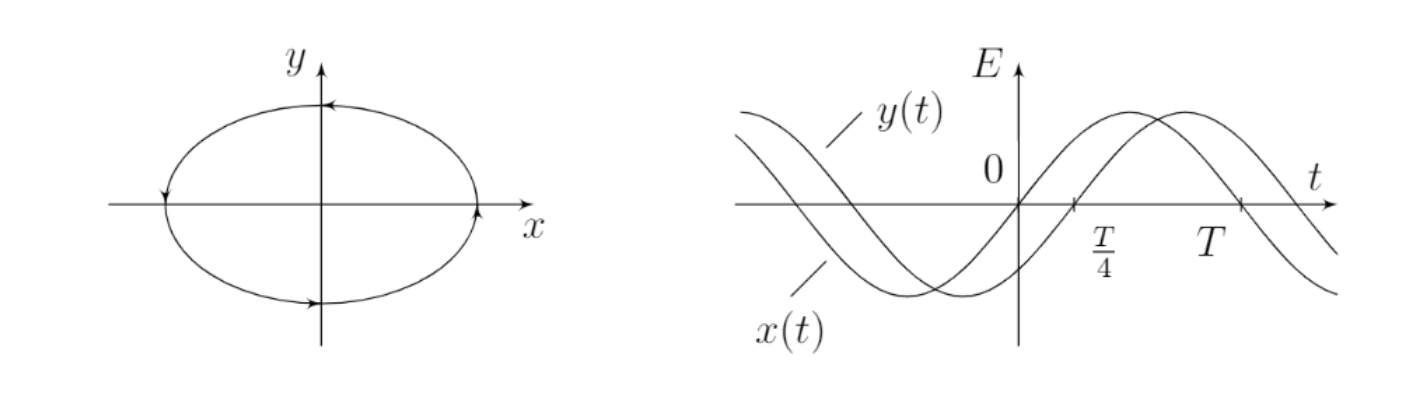
\includegraphics[width=0.8\textwidth]{ellipse.png}
\caption{Эллипс поляризации и графики синусоид}
\end{figure}

\subsection*{Вывод}
Мы провели несколько качественных эксперементов и узнали, как создавать и исследовать поляризованное излучение. Мы познакомились с линейной, круговой и эллиптической поляризацией.

\newpage

\subsection*{Ответы на контрольные вопросы}
\begin{enumerate}
    \item \textbf{Покажите, что при выполнении условия Брюстера отражённый и преломлённый лучи взаимно перпендикулярны.}

    При угле Брюстера $i_B$ отражённый и преломлённый лучи взаимно перпендикулярны. Согласно закону Брюстера:
    \[
    \tan i_B = \frac{n_2}{n_1}
    \]
    Согласно закону преломления:
    \[
    n_1 \sin i_B = n_2 \sin r
    \]
    При этом угол между отражённым и преломлённым лучами равен $90^\circ$, то есть:
    \[
    i_B + r = 90^\circ \Rightarrow r = 90^\circ - i_B
    \]
    Подставим в закон преломления:
    \[
    n_1 \sin i_B = n_2 \cos i_B \Rightarrow \tan i_B = \frac{n_2}{n_1}
    \]
    Что и требовалось доказать.

    \item \textbf{Как отличить свет с правой и с левой круговой поляризацией?}

    Свет с правой и левой круговой поляризацией можно отличить с помощью четвертьволновой пластинки ($\lambda/4$) и поляризатора. После прохождения через пластинку круговая поляризация преобразуется в линейную. Далее, поворачивая поляризатор, можно определить направление поляризации и, следовательно, отличить правую поляризацию от левой.

    \item \textbf{Неполяризованный свет проходит через двоякопреломляющую пластинку $\lambda/4$. Что можно сказать о поляризации света на выходе из пластинки?}

    Если на пластинку $\lambda/4$ падает неполяризованный свет, то на выходе получится частично поляризованный свет. Это происходит потому, что пластинка преобразует компоненты света, колеблющиеся в разных плоскостях, создавая между ними фазовый сдвиг $\pi/2$.

    \item \textbf{Как отличить естественный свет от света, поляризованного по кругу, и от смеси естественного света со светом, поляризованным по кругу?}

    Для различения используют поляризатор и $\lambda/4$ пластинку. Естественный свет не изменяет интенсивности при вращении поляризатора, круговая поляризация — также. Однако если перед поляризатором поставить пластинку $\lambda/4$, то круговая поляризация превратится в линейную и интенсивность будет меняться при вращении поляризатора. Смесь можно определить по частичному изменению интенсивности.

    \item \textbf{Объясните изменения интенсивности и цвета, наблюдаемые в опытах по интерференции поляризованных лучей.}

    При интерференции поляризованных лучей наблюдаются изменения интенсивности в зависимости от разности фаз и поляризации. Если лучи когерентны и имеют одинаковую поляризацию, то происходит интерференция. При разной поляризации интенсивность зависит от угла между поляризациями. Цветовые изменения обусловлены зависимостью интерференции от длины волны.

    \item \textbf{Почему свет от вечернего неба поляризован?}

    Поляризация света от неба объясняется рассеянием Рэлея. При рассеянии солнечного света молекулами атмосферы на угле $90^\circ$ к направлению солнечных лучей свет становится частично поляризованным. Вечером Солнце низко над горизонтом, и рассеянный свет, доходящий до наблюдателя, проходит через значительное количество атмосферы, усиливая эффект поляризации.

\end{enumerate}

\end{document}








% \lipsum[1-4]
% \begin{wrapfigure}{R}{5cm}
% \centering
% \includegraphics[width=0.20\textwidth]{rd.png}
% \caption{1}
% \end{wrapfigure}
% \lipsum[1-6]


% \begin{figure}[h]
% \begin{center}$
% \begin{array}{cccc}
% \includegraphics[width=0.20\textwidth]{rd.png}&
% \includegraphics[width=0.20\textwidth]{rd.png}&
% \includegraphics[width=0.20\textwidth]{rd.png}&
% \includegraphics[width=0.20\textwidth]{rd.png}\\
% (1) & (2) & (3) & (4)
% \end{array}$
% \end{center}
% \end{figure}
